\chapter{MODEL DEVELOPMENT} \label{label:modeldevelopment}

\graphicspath{{./figures/}}

\section{General}

\section{Physical Setup}
Being a salt water species, macroalgae cultivation occurs primarily in the ocean, with the exception of the initial stage of growth, where microscopic kelp spores are inoculated onto a thread in a small laboratory pool.
This thread is then wrapped around a large rope, which is placed in the ocean and generally suspended by buoys in one of two configurations: horizontal or vertical.
Thus far, I am primarily concerned with modeling the vertical rope case, in which the kelp plants extend radially outward from the rope in all directions, which are made up of a single frond (leaf), stipe (stem) and holdfast (root structure).
We consider a rectangular grid of such vertical ropes. 
Plants extending from each rope will shade both themselves and their neighbors to varying degrees based on the depth of the kelp, the rope spacing, the angle of incident light and the nature of scattering in the water.
In addition, light will be naturally absorbed by the water to varying degrees as determined by the clarity of the water.

\begin{figure}[H]
	\centering
	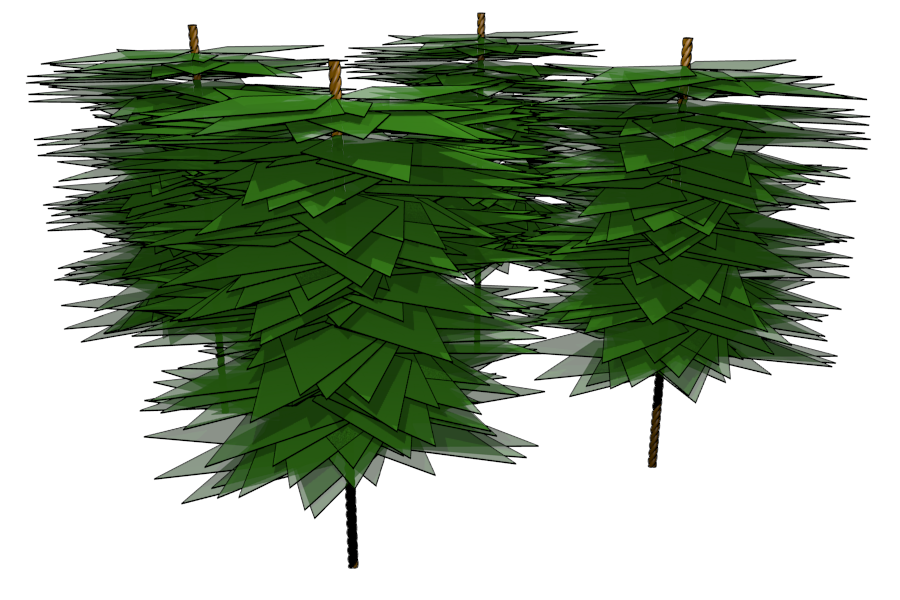
\includegraphics[width=3.5in]{kelp_array}
	\captionof{figure}{$4\times 4$ array of vertical kelp ropes}
\end{figure}
\section{Coordinate System}
%For all of our three dimensional analysis, we will use the absolute coordinate system defined in figure \ref{fig:3dcoords}.
In the following sections, we will wish to convert between Cartesian and spherical coordinates, which we will do using the following formulas.
\begin{align}
	\begin{split}
		x & = r\sin\phi\cos\theta \\
		y & = r\sin\phi\sin\theta \\
		z & = r\cos\phi \\
	\label{eqn:coords}
	\end{split}
\end{align}

%Therefore, for some function $f(x,y,z)$, we can write its derivative along a path in spherical coordinates in terms of Cartesian coordinates using the chain rule.
\begin{equation}
	\frac{\partial f}{\partial r} 
	=\frac{\partial f}{\partial x}\frac{\partial x}{\partial r} 
	+ \frac{\partial f}{\partial y}\frac{\partial y}{\partial r} 
	+ \frac{\partial f}{\partial z}\frac{\partial z}{\partial r}
\end{equation}
Then, calculating derivatives from \eqref{eqn:coords}, we get
\begin{equation}
	\frac{\partial f}{\partial r} 
	=\frac{\partial f}{\partial x}r\sin\phi\cos\theta
	+ \frac{\partial f}{\partial y}r\sin\phi\sin\theta
	+ \frac{\partial f}{\partial z}r\cos\phi
	\label{eqn:partials}
\end{equation}
\begin{figure}[H]
	\centering
	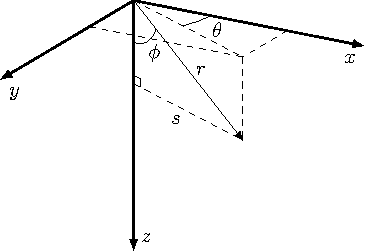
\includegraphics[width=3in]{3d_coords}
	\caption{Downward-facing right-handed coordinate system with radial distance $r$ from the origin, distance $s$ from the $z$ axis, zenith angle $\phi$ and azimuthal angle $\theta$}
	\label{fig:3dcoords}
\end{figure}

\section{Kelp Model}

\section{2D Model}
First, let us consider a 2D vertical slab of width $dz$ of a single rope with kelp extending from it.
We assume that the number (not mass) density of kelp plants, $\rho$ is initially uniform along the length of the rope.

\subsection{Frond shape}
\label{sec:shape}

\begin{figure}[H]
	\centering
	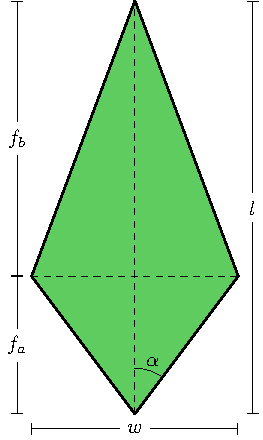
\includegraphics[width=2in]{frond}
	\captionof{figure}{Model frond diagram}
	\label{fig:frond}
\end{figure}

The frond is a kite with length $l$ from base to tip, and width $w$ from left to right.
 %In figure \ref{fig:frond}, the base is shown at the bottom and the tip is shown at the top.
 The shortest distance from the base to the diagonal connecting the left and right corners is called $f_a$, and the shortest distance from that diagonal to the tip is called $f_b$.
 Clearly,
 \begin{equation}
	 f_a + f_b = l
 \end{equation}
When considering a whole population with varying sizes, it is more convent to specify ratios than absolute lengths.
Let the following ratios be defined.
\begin{align}
	f_r &= \frac{l}{w} \\
	f_s &= \frac{f_a}{f_b}
\end{align}
These ratios are assumed to be consistent among the entire population, making all fronds geometrically similar.
With these definitions, the shape of the frond can be fully specified by $l$, $f_r$, and $f_s$.
It is possible, then, to redefine $w$, $f_a$ and $f_b$ as follows from the preceding formulas.

\begin{align}
	w &= \frac{l}{f_r} \\
	f_a &= \frac{lf_s}{1+f_s} \\
	f_b &= \frac{l}{1+f_s}
\end{align}

The angle $\alpha$, half of the angle at the base corner, will be important in our analysis.
Using the above equations,
\begin{equation}
	\alpha = \tan^{-1}\left(\frac{2f_rf_s}{1+f_s}\right)
\end{equation}

\section{Population Distribution}
\label{sec:dist}

\subsection{Superindividuals}

The kelp lifecycle model of which this work is part is based on the concept of
superindividuals, which are kelp fronds which represent a subpopulation of
identical fronds.

** WE HAVE TO CALCULATE LENGTH BEFORE CALCULATING STANDARD DISTRIBUTION **

At each depth $k$, we have $n$ superindividuals, indexed by $i$. Superindividual
$i$ has a frond area $a_{ki}$ and represents $n_{ki}$ individual fronds.

\subsection{Length Distribution}

Given the superindividual data, we calculate the mean $\mu$ and standard deviation $\sigma$ frond
lengths using the formulas:
\begin{equation}
  \mu_k = \frac{\ds \sum_{i=1}^N a_{ki}}{\ds \sum_{i=1}^N n_{ki}} 
\end{equation}
\begin{equation}
  \sigma_k = \frac{\ds \sum_{i=1}^N \left( a_{ki} - \mu_k \right)^2}{\ds \sum_{i=1}^N n_{ki}} 
\end{equation}

We then assume that frond lengths are normally distributed in each depth layer
with mean $\mu_k$ and standard deviation $\sigma_k$.

\subsection{Frond angle distribution}
\label{sec:angle_dist}
The frond angle varies according to the von Mises distribution, which is the periodic analogue of the normal distribution.
It is defined on $[-\pi,\pi]$ rather than $(-\infty,\infty)$.
It has two parameters, $\mu$ and $\kappa$, which shift and sharpen the distribution respectively.
%$\kappa$ can be considered analogous to $1/\sigma$ in the normal distribution.
Here, we use $\mu = \theta_w$ and $\kappa = v_w$.

The PDF for this distribution is
\begin{equation}
	P_{\theta_f}(\theta_f) = \frac{e^{(v_w)\cos(\theta_f-v_w)}}{2\pi I_0(v_w)}
\end{equation}
where $I_0(x)$ is the modified Bessel function of the first kind of order 0.
Notice that unlike the normal distribution, the von Mises distribution approaches a \textit{non-zero} uniform distribution as $\kappa$ approaches 0.
\begin{equation}
	\displaystyle \lim_{v_w \to 0}P_{\theta_f}(\theta_f) = \frac{1}{2\pi} \;\forall\, \theta_f \in [-\pi,\pi]
\end{equation}
The idea behind using this distribution is that with zero current velocity, the frond angles should be distributed uniformly, while as current velocity increases, they should be increasingly likely to be pointing in the direction of the current.
Note that $\theta_w$ and $v_w$ are functions of position.
For a given depth layer, we will use the average water velocity for that depth.

\begin{figure}[H]
	\centering
	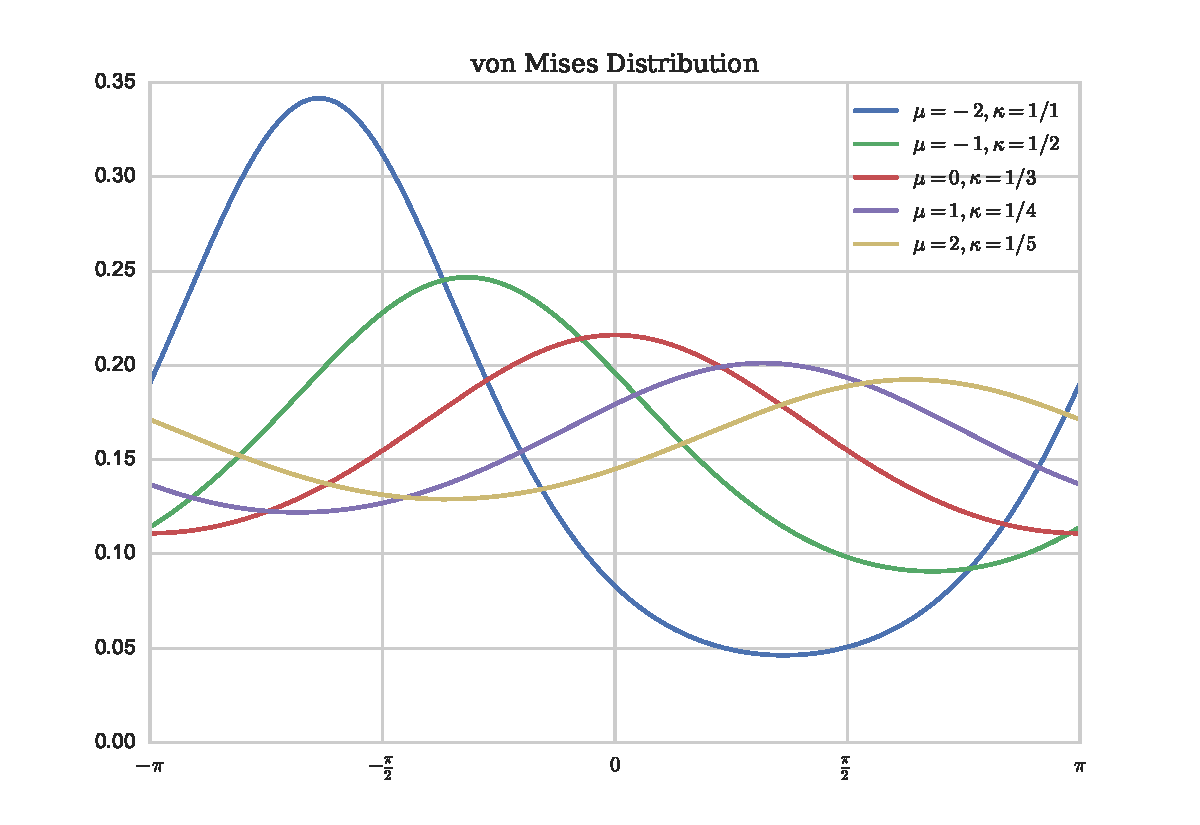
\includegraphics[width=\linewidth]{vonmises_2}
	\captionof{figure}{von Mises distribution for a variety of parameters}
	\label{fig:vonmises}
\end{figure}

\subsection{Combined 2D length-angle distribution}
\label{sec:2d_dist}
The previous two distributions are independent of one another. That is, the angle of the frond does not depend on the length, or vice versa.
Therefore, the probability of a frond simultaneously having a given frond length and angle is the product of their individual probabilities.

Given independent events $A$ and $B$,
\begin{equation}
	\label{eq:ind_prob}
	P(A \cap B) = P(A)P(B)
\end{equation}
Then the probability of frond length $l$ and frond angle $\theta_f$ coinciding is 
\begin{equation}
	P_{2D}(\theta_f,l) = P_{\theta_f}(\theta_f) \cdot L(l)
\end{equation}
A contour plot of this 2D distribution for a specific set of parameters is shown in figure \ref{fig:dist_2d}, where probability is represented by color in the 2D plane.
Darker green represents higher probability, while lighter beige represents lower probability.
In figure \ref{fig:kelp_sample}, 50 samples are drawn from this distribution and plotted.

It is important to note that if $P_{\theta_f}$ were dependent on $l$, the above definition of $P_{2D}$ would no longer be valid.
For example, it might be more realistic to say that larger fronds are less likely to bend towards the direction of the current.
In this case, \eqref{eq:ind_prob} would no longer hold, and it would be necessary to use the following more general relation.
\begin{equation}
	P(A \cap B) = P(A)P(B|A) = P(B)P(B|A)
\end{equation}
This is currently not taken into consideration in this model.

\begin{figure}[H]
	\centering
	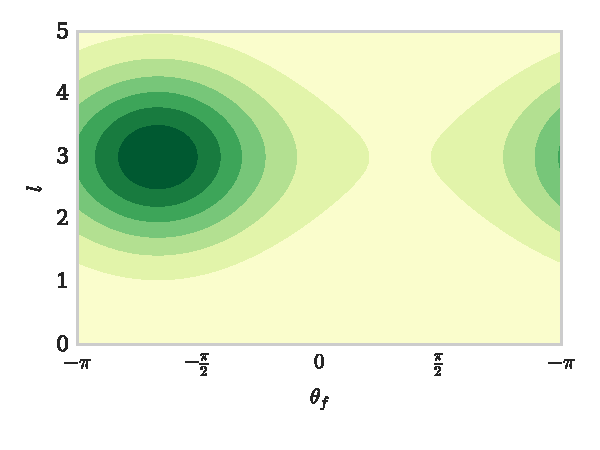
\includegraphics[width=\linewidth]{prob_2d}
	\vspace{-3em}
	\captionof{figure}{2D length-angle probability distribution with $\theta_w=2\pi/3,v_w=1$}
	\label{fig:dist_2d}
\end{figure}

\begin{figure}[H]
	\centering
	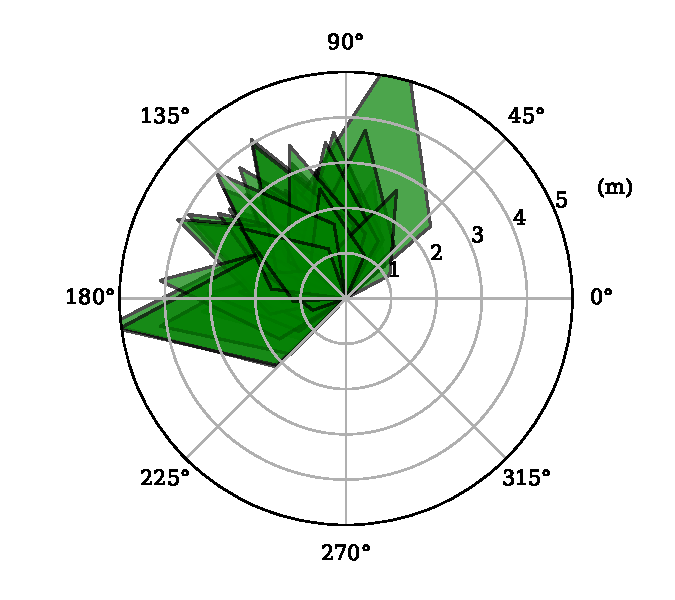
\includegraphics[width=\linewidth]{kelp_sample}
	\vspace{-2em}
	\captionof{figure}{A sample of 50 kelp fronds with length and angle picked from the distribution above with $f_s=0.5$ and $f_r=2$.}
	\label{fig:kelp_sample}
\end{figure}

\subsection{Relative coordinate system}
\label{sec:rel_coords}
To determine under what conditions a frond will shade a given point, we begin by describing the shape of the frond in Cartesian and then polar coordinates.
Of primary interest are the edges connected to the frond tip.
For convenience, we will use a relative coordinate system $(\theta',s)$ such that the line connecting the base to the tip is vertical, with the base at $(0,0)$.
The Cartesian analogue of this coordinate system, $(x',y')$, has the following properties.
\begin{align}
	x' &= s\cos\theta' \\ 
	y' &= s\sin\theta'
\end{align}
and
\begin{align}
	s &= \sqrt{x'^2+y'^2}
\end{align}
\vspace{-1em}
\begin{align}
	\theta' &= \atantwo(y, x)
\end{align}

\subsection{Functional description of frond edge}
With this coordinate system established, we can describe the outer two edges of the frond in Cartesian coordinates as a piecewise linear function connecting the left corner: $(-w/2,f_a)$, the tip: $(0,l)$, and the right corner: $(w/2,f_a)$.
This function has the form
\begin{equation}
	y'_f(x') = l-\sign(x')\frac{f_b}{w/2}x'
\end{equation}
where
\begin{align}
	\sign(x) = 
	\begin{cases}
		1 & x > 0 \\
		0 & x = 0 \\
		-1 & x < 0 \\
	\end{cases}
\end{align}

%Using the equations in section \ref{sec:rel_coords}, this can be written in polar coordinates after some rearrangement as
\begin{equation}
	s_f'(\theta') = \frac{l}{\sin\theta' + S(\theta')\frac{2f_b}{w}\cos\theta'}
\end{equation}
where
\begin{equation}
	S(\theta') = \sign(\theta'-\pi/2)
\end{equation}

%Then, using the relationships in section \ref{sec:shape}, we can rewrite the above equation in terms of our frond ratios $f_s$ and $f_r$.
\begin{equation}
	\label{eq:rf_rel}
	s_f'(\theta') = \frac{l}{\sin\theta' + S(\theta')\frac{2f_r}{1+f_s}\cos\theta'}
\end{equation}

\subsection{Absolute coordinates}
\label{sec:abs_coords}
To generalize to a frond pointed at an angle $\theta_f$, we will use the coordinate system $(\theta,s)$ such that
\begin{equation}
	\theta = \theta' + \theta_f - \frac{\pi}{2}
\end{equation}
Then, for a frond pointed at the arbitrary angle $\theta_f$, the function for the outer edges can be written as 
\begin{equation}
	\label{eq:rf_abs}
	s_f(\theta) = s_f'\left(\theta - \theta_f + \frac{\pi}{2} \right)
\end{equation}


\subsection{Conditions for occupancy}
Consider a fixed frond of length $l$ at an angle $\theta_f$. The point
$(\theta,s)$ is occupied by the frond if
\begin{align}
	\left|\theta_f - \theta \right| < \alpha
	\shortintertext{and}
	s < s_f(\theta)
\end{align}

Equivalently, letting the point $(\theta,s)$ be fixed, a frond occupies the point if the following conditions are satisfied.
\begin{align}
	\theta - \alpha < \theta_f < \theta + \alpha
	\label{eqn:rs_th}
	\shortintertext{and}
	l > l_{min}(\theta,s)
	\label{eqn:rs_l}
\end{align}
where
\begin{equation}
	l_{min}(\theta,s) = s \cdot \frac{l}{s_f(\theta)}
\end{equation}


Then, considering the point to be fixed, \eqref{eqn:rs_th} and \eqref{eqn:rs_l} define the spacial region $R_s(\theta,s)$ called the ``occupancy region for $(\theta,s)$'' with the property that if the tip of a frond lies within this region (i.e. $(\theta_f,l) \in R_s(\theta,s)$), then it occupies the point.
$R_s(3\pi/4,3/2)$ is shown in blue in figure \ref{fig:shade_area} and the smallest possible occupying fronds for several values of $\theta_f$ are shown in various colors.
Any frond longer than these at the same angle will also occupy the point.

\begin{figure}[H]
	\centering
	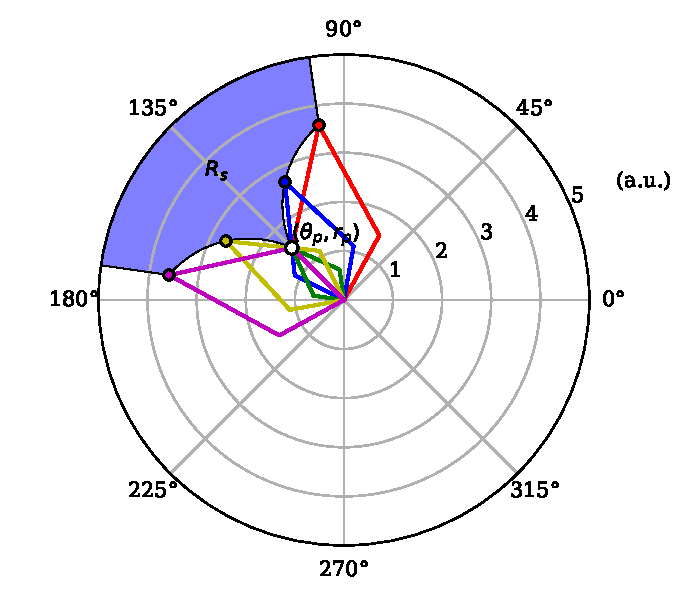
\includegraphics[width=\linewidth]{shade_area}
	\vspace{-2em}
	\captionof{figure}{Outlines of minimum-length fronds for a variety of angles to occupy the point $(\theta,s)=(3\pi/4,3/2)$}
	\label{fig:shade_area}
\end{figure}

\subsection{Probability of occupancy}
NOT SO SURE ABOUT THIS
%We are interested in the probability that, given a fixed point $(\theta,s)$, values of $l$ and $\theta_f$ chosen from the distributions described in section \ref{sec:dist} will fall in the occupancy region.
%$This is found by integrating $P_{2D}$ over the occupancy region for $(\theta,s)$, as depicted in figure \ref{fig:cart_shade}.

\begin{figure}[H]
	\centering
	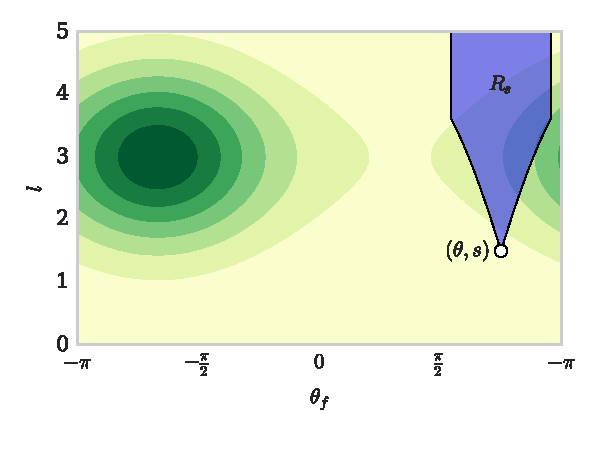
\includegraphics[width=\linewidth]{cart_shade}
	\vspace{-3em}
	\captionof{figure}{Contour plot of $P_{2D}(\theta_f,l)$ overlayed with the
    region in the $\theta_f-l$ plane which results in a frond occupying the point $(\theta,s)=(3\pi/4,3/2)$}
	\label{fig:cart_shade}
\end{figure}

Now, we are able to define the probability of a frond occupying the point $(\theta,s)$ at a depth $z$ at time $t$ by
\begin{align}
		P_k(\theta,s,z,t)	&= \iint_{R_s(\theta,s,z,t)}
								P_{2D}(\theta_f,l)
								\;dl\;d\theta_f \nonumber \\
							&= \int_{\theta-\alpha}^{\theta+\alpha} 
								\int_{l_{min}(\theta_f,z,t)}^\infty
								P_{2D}(\theta_f,l)
								\;dl\;d\theta_f
\end{align}

\begin{figure}[H]
	\centering
	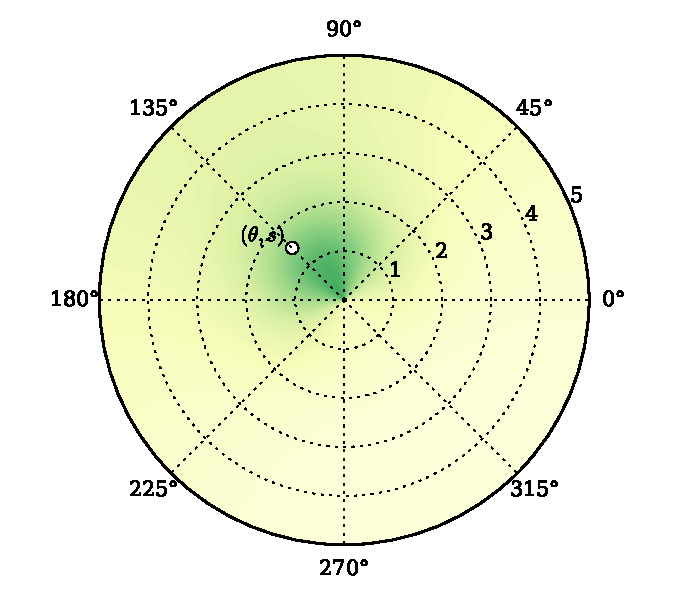
\includegraphics[width=\linewidth]{prob_shade}
	\vspace{-2em}
	\captionof{figure}{Contour plot of the probability of occupying sampled at 121 points using $\theta_f=2\pi/3,v_w=1$}
	\label{fig:prob_shade}
\end{figure}


\section{Light Model}

\subsection{Background}
In terms of optical quantities, our primary interest is in the radiance at each point from all directions, which affects the photosynthetic rate of the kelp, and therefore the total amount of biomass producible in a given area as well as the total nutrient absorption potential.
The equation governing the radiance throughout the system is known as the Radiative Transfer Equation (RTE), which has been largely unutilized in the fields of oceanography and aquaculture.
Meanwhile, it has been studied extensively in two fields: stellar astrophysics and computer graphics.
In its full form, radiance is a function of 3 spatial dimensions, 2 angular dimensions, and frequency, making for an incredibly complex problem.
Thus far, I have ignored the dependence on frequency, and have only considered monochromatic radiation.
The RTE states that along a given path, radiance is decreased by absorption and scattering out of the path, while it is increased by emission and scattering into the path.
In our situation, emission is negligible, owing only perhaps to some small luminescent phytoplankton or some such anomaly, and can therefore be safely ignored.
\subsection{Optical Definitions}
One of the most fundamental quantities in optics is radiant flux $\Phi$, which is the has units of energy per time.
The quantity of primary interest in modeling the light field is radiance $R$, which is defined as the radiant flux per steradian per projected surface area perpendicular to the direction of propagation of the beam.
That is,
\begin{equation}
	R = \frac{d^2\Phi}{dA d\omega}
\end{equation}
We must now define a few inherent optical properties (IOPs) which depend only on the medium of propagation.

Consider a beam of light traveling through the water in the direction $\underline{\omega} = (\theta,\phi)$.
As it travels, there will be some decrease in the radiance due to scattering and absorption.
Let $a_w$ and $b_w$ be the coefficients of absorption and scattering respectively due solely to the water.
Similarly, define $a_k$ and $b_k$ to be the absorption and scattering coefficients due solely to kelp.
The loss due to scattering or absorption, whether by kelp or water, is proportional to radiance, and $a_w,b_w,a_k,b_k$ all have units of inverse meters.

There will also be some gain into the path of the beam due to scattering from other directions, as determined by the \textit{volume scattering function},
$\displaystyle \beta(\Delta\theta): [0,\pi) \rightarrow \R^+$, which gives the proportion of incident radiance scattered at an angle $\Delta\theta$ from its original direction due to only water.
The units of $\beta$ are $\mbox{m}^{-1}\mbox{rad}^{-2}$.

For convenience, let $\displaystyle \beta(\underline{\omega}_1,\underline{\omega}_2) = \beta\left(\cos^{-1}\left(\frac{\underline{\omega}_1\cdot\underline{\omega}_2}{\norm{\underline{\omega}_1}\norm{\underline{\omega}_1}}\right)\right)$. 

\subsection{PDE}
From the discussion above, our governing PDE, the radiative transfer equation, can be written as
\begin{equation}
	\frac{\partial R}{\partial r} = 
	- c_kP_k - (1-P_k)c_w
	+ \iint_{4\pi}
	\beta_k(\underline{\omega},\underline{\omega}')
	R(x,y,z,\underline{\omega}')\,d\underline{\omega}'
	\label{eqn:rte1}
\end{equation}
where $c_k = a_k + b_k$, $c_w = a_w + b_w$, and $\underline{\omega}' \neq \underline{\omega}$.

%Using \eqref{eqn:partials}, this can be rewritten in terms of Cartesian coordinates as
\begin{align}
	\begin{split}
	\frac{\partial R}{\partial x}\sin\phi \cos\theta 
	&+ \frac{\partial R}{\partial y}\sin\phi \sin\theta
	+ \frac{\partial R}{\partial z}\cos\phi \\ 
	&= - c_kP_k - (1-P_k)c_w \\
	&+ \iint_{4\pi}
	\beta_k(\underline{\omega},\underline{\omega}')
	R(x,y,z,\underline{\omega}')\,d\underline{\omega}'
	\end{split}
	\label{eqn:rte2}
\end{align}
\subsection{Boundary Conditions}
Though I have determined the PDE which governs the behavior of the radiance in the domain, I am lacking a full set of appropriate boundary conditions for the system.

Since we have one derivative per spatial dimension, we need one boundary condition per spatial dimension as well.
For $x$ and $y$, it may be favorable to use periodic boundary conditions in order to simulate a large array of kelp ropes spread out over the surface of the ocean.
It is worth mentioning, though, that special consideration may be necessary in order to account for smaller rope grids, for which edge effects neglected by periodic boundary conditions may become relevant.

It is the $z$ boundary condition which is puzzling me.
We should be able to make reasonable assumptions about the incident radiation from the atmosphere, though it seems that this is not sufficient.
We can only use atmospheric conditions for downwelling radiation.
It doesn't seem reasonable that radiance from above would have a direct effect on upwelling radiation.
In this sense, we only have half of the boundary condition that we need.
Then it seems that the other half should come from the bottom of the simulation.
But I would like to avoid putting any kind of specifically reflective or absorptive boundary on the \textit{bottom} of the simulation box, since the ocean would likely be much larger than the kelp.
In this case, it would be of interest to find some bottom boundary condition which allows for the free flow of radiance in and out of the bottom boundary.

\section{Irradiance and Flux}
Assume that the radiance $R_{ijklm}$ is known at all angles $(\theta_l,\phi_m)$ at all points $(x_i,y_j,z_k)$ on a Cartesian grid.
Since we seek to calculate the radiant flux $\Phi$ through each frond (i.e. the quantity of solar energy that it receives per unit time), we must first calculate the irradiance as an intermediate quantity.

\subsection{Formulation}
The downward irradiance $E$  at a point $(x,y,z)$ is defined as
\begin{align}
	E(x,y,z) &= \iint_{2\pi} R(x,y,z;\theta,\phi)\,d\theta d\phi.
\end{align}
Then
\begin{equation}
	E_{ijklm}= \sum_{\substack{l=1 \\ \theta_l < \pi/2}}^{M_\theta}\sum_{m=1}^{M_\phi} R_{ijklm}
\end{equation}

Let $F(\theta_f,l)$ be the 2D spatial region occupied by a frond of length $l$ pointed in the direction $\theta_f$.
\begin{equation}
	\Phi = \iint_{F(\theta_f,l} E(x,y,z)\,dxdy
\end{equation}

\subsubsection{Calculation}
Note that this region is kite shaped, which doesn't make for a straightforward analytical or numerical integral.
Thus, we introduce the transformation $\tau$ that maps a point $(u,v)$ on the unit square to the corresponding point $(x,y)$ on a vertical frond $F(\frac{\pi}{2},l)$
In particular, we have $\tau(-1,-1) = (0,0)$, $\tau(1,1) = (0,l)$, $\tau(1,-1) = (w/2,f_a)$, and $\tau(-1,1) = (-w/2,f_a)$.
In full, $\tau(u,v) = (x,y)$, where
\begin{align}
	x &= \frac{l(u-v)}{4f_r} \\
	y &= -\left(\frac{l}{4}\right) \frac{f_s(u-1)(v+1) - (u+1)(2f_s + v + 1)}{1+f_s}
\end{align}

The Jacobian of $\tau$, then, is given by
\begin{equation}
	J = \left(\frac{l}{16f_r}\right) \frac{u + v + 2 - f_s(u-1)(v-1)}{1+f_s} \\
\end{equation}

Note that we can generalize $\tau$ to map to a frond at any angle $\theta_f$ by introducing the 2D rotation matrix.
We can rotate a point $\underline{r}_1 = (x_1,y_1) \in \R^2$ to a new point $\underline{r}_2 = (x_2,y_2) \in \R^2$ by an angle $\theta$ about the origin by pre-multiplying by the rotation matrix $W_{\theta}$, where
\begin{equation}
	W_{\theta} = \left[ \begin{array}{cc}
		\cos\theta & -\sin\theta \\
		\sin\theta & \cos\theta \\
	\end{array} \right]
\end{equation}
That is
\begin{equation}
	\underline{r}_2 = W_{\theta} \underline{r}_1
\end{equation}

Let $T_{\theta} = W_{\theta} \tau$.
Then, $T_{\theta_f'}: [-1,1]\times[-1,1] \to F_{\theta_f}$ transforms $(u,v)$ on the unit square to the corresponding point $(x,y)$ on the frond with base at the origin pointing in the direction $\theta_f$

\subsubsection{Gaussian Quadrature}
With this in mind, we can use a Gaussian quadrature on the unit square to approximate the integral over the surface of a frond by summing the values for $E$ at the 4 points $\displaystyle\left\{T_{\theta_f'}\left(\pm\sqrt{\frac{1}{3}}\right)\right\}$. Although these points likely do not fall on our Cartesian grid for an arbitrary frond angle, we can use bilinear interpolation to approximate the value of $E$ at these points.
I have yet to study the efficiency and accuracy of this technique for calculating flux.

%%% FROM RTE 2D PAPER
\subsection{Radiative Transfer}
Let $n$ be the number of spatial dimensions for the problem (i.e., 2 or 3).
Let $x \in \RR^n$.
Let $\Omega$ be the unit sphere in $\RR^n$.
Let $\omega \in \Omega$ be a unit vector in $\RR^n$.
Let $L(x,\omega)$ denote \textit{radiance} position $x$ in the direction $\omega$.
Let $I(x)$ denote \textit{irradiance} at position $x$.
Let $P_k(x)$ be the probability density of kelp at position $x$.
Let $a_w$ and $a_k$ be the absorption coefficients of water and kelp respectively.
Let $b_w$ and $b_k$ be the scattering coefficients of water and kelp respectively.
Then we define the effective absorption and scattering coefficients as
\begin{align}
	\label{eq:abs}
	a(x) &= P_k(x) a_k + (1-P_k(x)) a_w \\
	\label{eq:sct}
	b(x) &= P_k(x) b_k + (1-P_k(x)) b_w
\end{align}
Then, the Monochromatic Time-Independent Radiative Transfer Equation (RTE) is
\begin{equation}
    \tag{RTE}
    \label{eq:rte}
    \begin{aligned}
        \omega \cdot \nabla_x L(x,\omega) &= -(a(x) + b(x)) L(x,\omega) \\
        &\qquad + b \int_\Omega \beta(\omega \cdot \omega') L(x,\omega')\, d\omega'
    \end{aligned}
\end{equation}

Note that in 2 spatial dimensions, this is a 3-dimensional problem ($x,y,\theta$).
Likewise, in 3 spatial dimensions, it is a 5-dimensional problem ($x,y,z,\theta,\phi$).

In this paper, we consider only the 2-dimensional problem, with the hope that sufficiently robust solution techniques for the 2-dimensional problem will be effective in the solution of the 3-dimensional problem as well.

\subsection{Boundary Conditions}
We assume that the downwelling light from the surface is known, and is defined to be uniform in space by the Dirichlet boundary condition
\begin{equation}
    L(x,0,\theta) = f(\theta), \quad \mbox{for} \quad \theta \in [0,\pi).
    \label{eq:surf_bc}
\end{equation}

Note that we cannot apply the same idea to upwelling light at the surface, as it cannot be specified from information about the atmospheric light field.
Therefore, we apply the PDE at $y=0$ for $\theta \in [\pi,2\pi)$.

At $y=1$, we assume no upwelling light.
That is,
\begin{equation}
    L(x,0,\theta) = 0, \quad \mbox{for} \quad \theta \in [\pi,2\pi).
    \label{eq:bottom_bc}
\end{equation}

As with the upper $y$-boundary, we apply the PDE for $\theta \in [0,\pi)$ so as not to prohibit downwelling light.

In the horizontal direction, we assume periodic boundary conditions.
Assuming that a single discrete group of plants is being simulated, adjusting the width of the domain effectively modifies the spacing between adjacent groups of plants.

\section{System of Linear Equations}

\subsection{Discretization}
In order to solve \eqref{eq:rte} numerically, we discretize the spatial derivatives using 2nd order finite difference approximations, and we discretize the integral according to the Legendre-Gauss quadrature, as described in \cite[Chapter 2]{chandrasekhar_radiative_1960}.
With this in mind, in order to create a spatial-angular grid with $n_x,n_y,
n_z, n_\theta$, and $n_\phi$ discrete values for $x, y, z, \theta$, and $\phi$
respectively, we use a uniform rectangular grid with spacings $dx = (x_{max} -
x_{min})/n_x$, etc. For the spatial variables, we have $x_i = x_{min} + (i-1) \cdot dx$
for $i=1,\ldots, n_x$. Then, $x_{n_x} = x_{max} - dx$.

Now, the angular grid requires a slight modification to account for the poles.
For $l = 1, \ldots, n_{\theta}$, $m = 2, \ldots, n_{\phi}-1$, we have
$(\theta_l, \phi_m)$ defined as before. Then, the values of variables at
$\phi=0, \phi=\pi$ are stored separately.

% Then, we have the grid
% \begin{align}
%     x_i &= (i-1)\,dx, &\quad i=1,\ldots,n_x \\
%     y_j &= (j-1)\,dy, &\quad j=1,\ldots,n_y \\
%     \theta_k \,\, \mbox{s.t.}\,\,
%     &P_{n_\theta}(\theta_k/\pi-1) = 0, &\quad k=1,\ldots,n_\theta
% \end{align}

In the same notational vein, let \\[-1em]
\begin{align}
    \beta_{kl} &= \beta(\abs{\theta_k-\theta_l}), \\
    a_{ij} &= a(x,y) \\
    b_{ij} &= b(x,y)
\end{align}

where $\abs{\cdot}$ is periodic as in \eqref{eq:rte}.

For the spatial interior of the domain, we use the 2nd order central difference formula (CD2) to approximate the derivatives, which is
\begin{equation}
    \tag{CD2}
    f'(x) = \frac{f(x+dx)-f(x-dx)}{2dx} + \mathcal{O}(dx^3).
\end{equation}

When applying the PDE on the upper or lower boundary, we use the forward and backward difference (FD2 and BD2) formulas respectively.
Omitting $\mathcal{O}(dx^3)$, we have
\begin{equation}
    \tag{FD2}
    \label{eq:FD2}
    f'(x) = \frac{-3f(x)+2f(x+dx)-f(x+2dx)}{2dx}
\end{equation}
\begin{equation}
    \tag{BD2}
    \label{eq:BD2}
    f'(x) = \frac{3f(x)-2f(x-dx)+f(x-2dx)}{2dx}
\end{equation}

As for the angular integral, we substitute a weighted finite sum of the function evaluated at the angular grid points.
For each $k$, let $a_k$ be the appropriate Legendre-Gauss weight according to \cite[Chapter 2]{chandrasekhar_radiative_1960}.
Then, applying the change of variables theorem to transform from the standard quadrature interval $[0,1]$ to the correct angular interval $[0,2\pi]$, we have
\begin{equation}
    \tag{LG}
    \int_0^{2\pi} f(\theta)\,d\theta \approx \pi\sum_{k=1}^n a_k f(\theta_k)
\end{equation}

\subsection{Difference Equation}
%Given the above discrete approximations, the difference equation for \eqref{eq:rte} in the spatial interior of the domain is
\begin{align}
    \label{eq:diffeq}
    \begin{split}
    0 &= \frac{1}{2dx}\left(L_{i+1,j}^k - L_{i-1,j}^k\right) \cos\theta_k
    - \pi b \sum_{\substack{l=1\\ l\neq k}}^{n_\theta} a_l\beta_{kl}L_{ij}^l \\
    &+ \frac{1}{2dy}\left(L_{i,j+1}^k - L_{i,j-1}^k\right) \sin\theta_k
    + (a_{ij} + b_{ij})L_{ij}^k
    \end{split}
\end{align}

%Similarly, we discretize using \eqref{eq:FD2} and \eqref{eq:BD2} at the boundaries.
For example, when $j=1$, we have
\begin{align}
    \label{eq:diffeq_bc}
    \begin{split}
    &\quad0 = \frac{1}{2dx}\left(L_{i+1,j}^k - L_{i-1,j}^k\right) \cos\theta_k
    - \pi b \sum_{\substack{l=1\\ l\neq k}}^{n_\theta} a_l\beta_{kl}L_{ij}^l \\
	&+ \frac{1}{2dy}\left(4L_{i,j+1}^k - L_{i,j+2}^k\right) \sin\theta_k
	+ (a_{ij} + b_{ij} -\frac{3}{2dy})L_{ij}^k
    \end{split}
\end{align}

Note that when discretizing the integral, we exclude the $l=k$ term of the sum.
This is because that term corresponds to ``scattering'' straight ahead ($\Delta\theta=0$), which is in fact not scattering at all.
Whether some adjustment to the quadrature is necessary to account for this is unclear.

\subsection{Structure of Linear System}
For each $(i,j,k)$, we have a distinct equation with $4+n_\theta$ variables.
This corresponds to a sparse matrix equation $Ax=b$, each row having $4+n_\theta$ nonzero entries.
Note that $b$ is zero at each row except those which correspond to boundary conditions in $y$.

Each element in $x$ and $b$ correspond to a particular triple $(i,j,k)$, as are each row and column of the coefficient matrix $A$.
In some sense, when we create this linear system, we are unwrapping a 3-dimensional quantity (radiance) into a 1-dimensional vector (the solution, $x$).
Different orders in which the equations are listed can be chosen to generate equivalent systems, so long as the ordering is consistent in $A,b$, and $x$.

The most obvious way to order the equations is to do so via a triple \texttt{for} loop, which has the effect of creating blocks in the matrix corresponding to planes in $(x,y,\theta)$ space.
For example, if the equations are ordered such that the outer \texttt{for} loop is over $x$, and the inner two are over $y$ and $\theta$, then the first $(n_y n_\theta)$ rows of the matrix correspond to the equations for $i=1$.

By switching the order of the \texttt{for} loops, we can generate 6 equivalent matrix systems, each of which can be identified with a permutation of the triple $(0,1,2)$, where 0 corresponds to $x$, 1 corresponds to $y$, and 2 corresponds to $\theta$, and the order of the numbers indicates the order in which the loops were nested, from outer to inner.

The coefficient matrices $A$, generated by each of these choices are shown below for a trivially small system with $n_x=n_y=n_\theta=6$.
Each black square represents a nonzero entry, whereas gray lines are purely for visual aid.

\pagebreak
